% Options for packages loaded elsewhere
\PassOptionsToPackage{unicode}{hyperref}
\PassOptionsToPackage{hyphens}{url}
%
\documentclass[
]{article}
\usepackage{amsmath,amssymb}
\usepackage{lmodern}
\usepackage{ifxetex,ifluatex}
\ifnum 0\ifxetex 1\fi\ifluatex 1\fi=0 % if pdftex
  \usepackage[T1]{fontenc}
  \usepackage[utf8]{inputenc}
  \usepackage{textcomp} % provide euro and other symbols
\else % if luatex or xetex
  \usepackage{unicode-math}
  \defaultfontfeatures{Scale=MatchLowercase}
  \defaultfontfeatures[\rmfamily]{Ligatures=TeX,Scale=1}
  \setmainfont[]{Arial}
\fi
% Use upquote if available, for straight quotes in verbatim environments
\IfFileExists{upquote.sty}{\usepackage{upquote}}{}
\IfFileExists{microtype.sty}{% use microtype if available
  \usepackage[]{microtype}
  \UseMicrotypeSet[protrusion]{basicmath} % disable protrusion for tt fonts
}{}
\makeatletter
\@ifundefined{KOMAClassName}{% if non-KOMA class
  \IfFileExists{parskip.sty}{%
    \usepackage{parskip}
  }{% else
    \setlength{\parindent}{0pt}
    \setlength{\parskip}{6pt plus 2pt minus 1pt}}
}{% if KOMA class
  \KOMAoptions{parskip=half}}
\makeatother
\usepackage{xcolor}
\IfFileExists{xurl.sty}{\usepackage{xurl}}{} % add URL line breaks if available
\IfFileExists{bookmark.sty}{\usepackage{bookmark}}{\usepackage{hyperref}}
\hypersetup{
  pdftitle={La raport intermédiaire},
  pdfauthor={Antoine Viguié, Aymane Berriane, Christian Alvarez Leon, Meng Wang, Yu PENG},
  hidelinks,
  pdfcreator={LaTeX via pandoc}}
\urlstyle{same} % disable monospaced font for URLs
\usepackage[margin=1in]{geometry}



\usepackage{longtable,booktabs,array}
\usepackage{calc} % for calculating minipage widths
% Correct order of tables after \paragraph or \subparagraph
\usepackage{etoolbox}
\makeatletter
\patchcmd\longtable{\par}{\if@noskipsec\mbox{}\fi\par}{}{}
\makeatother
% Allow footnotes in longtable head/foot
\IfFileExists{footnotehyper.sty}{\usepackage{footnotehyper}}{\usepackage{footnote}}
\makesavenoteenv{longtable}
\setlength{\emergencystretch}{3em} % prevent overfull lines
\providecommand{\tightlist}{%
  \setlength{\itemsep}{0pt}\setlength{\parskip}{0pt}}
\setcounter{secnumdepth}{5}
\usepackage{booktabs}
\usepackage{amsthm}

%使用中文要使用这个包
\usepackage{ctex}

\usepackage{graphicx}
\graphicspath{{images/}} %表示图片在当前目录下的images目录

%封面====================================================================================================================
\usepackage{pdfpages}
%=========================================================================================================================

%重新命名=================================================================================================================

%\renewcommand{\bibname}{你的BIBLIOGRAPHY}
%\renewcommand{\abstractname}{你的ABSTRACT}

\renewcommand{\refname}{RÉFERENCES}

%\renewcommand{\chaptername}{Chapitre}

%\usepackage{titlesec}

%\usepackage{lipsum}

%\titleformat{\chapter}[display]{\normalfont\bfseries}{}{0pt}{\Large}

%标题命名
\renewcommand{\contentsname}{SOMMAIRE}

%图命名
\renewcommand{\figurename}{Figure}

%在toc中包含reference :https://tex.stackexchange.com/questions/57427/how-to-add-printindex-to-tableofcontents
\usepackage{makeidx}
\makeindex
\usepackage[nottoc]{tocbibind}

%toc 没有headers
\addtocontents{toc}{\protect\thispagestyle{empty}}

%=========================================================================================================================


%页眉页脚==================================================================================================================

%\fancyhead[R]{\kaishu 中国矿业大学~(北京) 硕士学位论文}
%\lhead{page \thepage\ of \pageref{LastPage}}
%\fancyhead[RO,LE]{\CJKfamily{hei} \bfseries \LaTeX{} 排版系统}
%\fancyhead[LO,RE]{\CJKfamily{hei>} \bfseries \leftmark}
%\renewcommand{\headrule}{\hrule width\headwidth \vspace{1.5pt}\hrule width\headwidth} % 所谓的文武线



%定义页眉页脚 fancyhdr 包
\usepackage{fancyhdr}
\pagestyle{fancy}

%默认清除所有的页眉和页脚设置
\fancyhf{} %清空页眉页脚 这是个更底层的命令

%设置页眉高度
\setlength\headheight{40pt}

%多行
%\fancyhead[c]{From: Frank\\To: Michel}

% 使用tabular 多行对齐
% \rhead{
    % \begin{tabular}[b]{l@{}}
        % Page: \thepage\\\today
    % \end{tabular}
    % }
\lhead{
\includegraphics[height=30pt]{ecole.png}}
\rfoot{\thepage}

%页眉横线
%\renewcommand\headrulewidth{0pt} %隐藏页眉横线
\renewcommand{\headrule}{\hrule width\headwidth \vspace{1.5pt}\hrule width\headwidth} % 所谓的文武线

%==========================================================================================================================

\makeatletter
\def\thm@space@setup{%
  \thm@preskip=8pt plus 2pt minus 4pt
  \thm@postskip=\thm@preskip
}
\makeatother

% 让url连接变为脚注
\renewcommand{\href}[2]{#2\footnote{\url{#1}}}
\ifluatex
  \usepackage{selnolig}  % disable illegal ligatures
\fi

%natbib 选项

\usepackage[]{natbib}
\bibliographystyle{plainnat}



\title{La raport intermédiaire}
\author{Antoine Viguié, Aymane Berriane, Christian Alvarez Leon, Meng Wang, Yu PENG}
\date{2020-12-07}

%==========================================================================================================================================
\begin{document}





%插入封面=================================================================
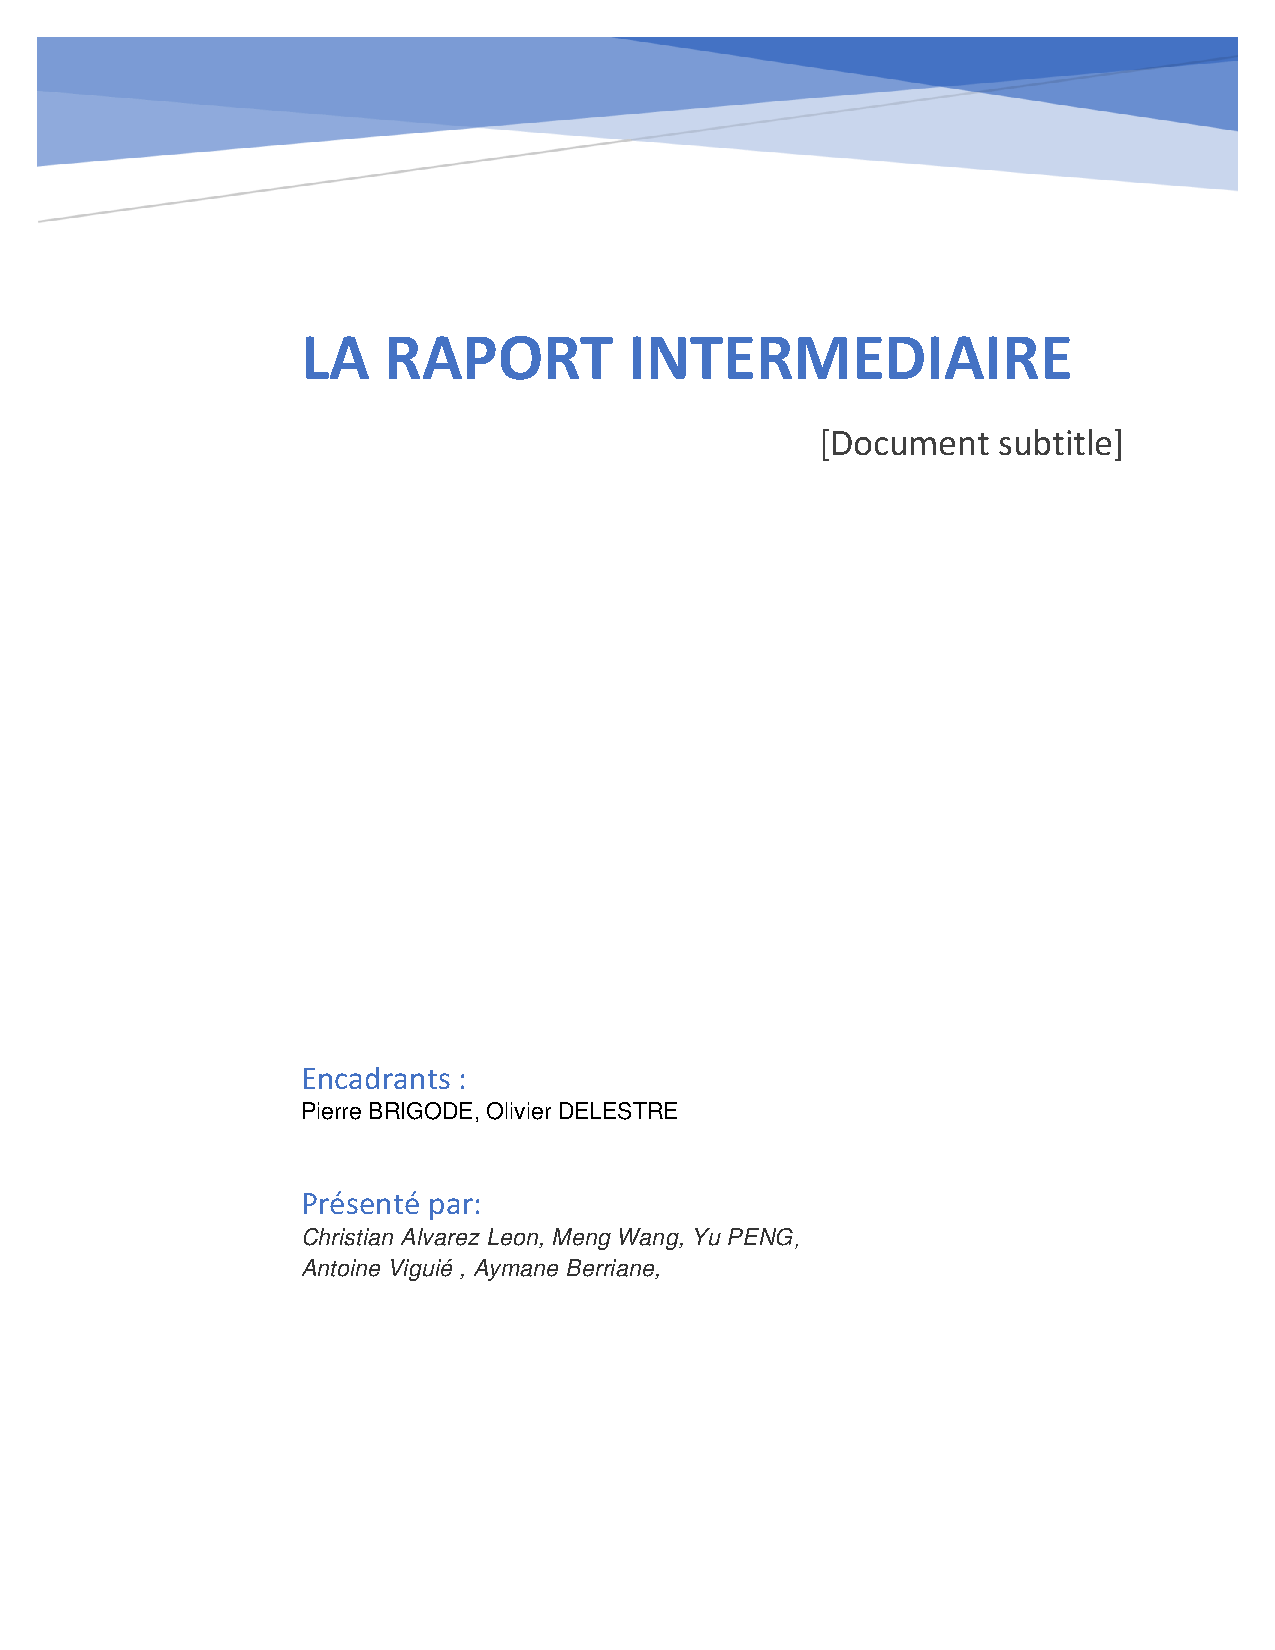
\includepdf{images/COVERPAGE.pdf}
%=======================================================================

%插入标题=================================================================
%%%\maketitle
%%=======================================================================

%加空白页但又heater
%\newpage
%\mbox{}
%\newpage



{
\setcounter{tocdepth}{2}
\tableofcontents
}


\newpage

\hypertarget{introduction}{%
\section{Introduction}\label{introduction}}

On observe régulièrement sur la Côte d'Azur, notamment à l'automne, de forts épisodes pluvieux, pouvant engendrer des crues. Par exemple, le 23 novembre 2019, des inondations exceptionnelles se sont produites sur la Côte d'Azur et ont inondé les plaines alluviales de l'Argens, de la Siagne et de la Brague notamment. Plus récemment, début octobre 2020, les vallées de la Roya, de la Vésubie ont été ravagées par des inondations, avec 500 mm relevés pendant l'épisode à Saint-Martin-Vésubie, du jamais vu à cette station depuis les relevés météorologiques. En raison de la nature destructrice des inondations, des recherches hydrologiques sur les bassins versants doivent être menées pour prendre les mesures d'anticipation et de protection de la population. Ceci nécessite par exemple de mesurer le débit sur des sections de cours d'eau non instrumentées en appareils de mesure. Dans notre projet, le but est de calculer le débit d'une section du canal de la Siagne par le logiciel Fudaa-LSPIV. Celui-ci permet de traiter des séquences d'images ou des vidéos d'écoulements pour calculer les champs de vitesse de surface et débit de la section choisie. Ce logiciel peut s'avérer utile pour mesurer le débit de sections de rivières avec un fort courant et de nombreux objets flottants, car les méthodes classiques seraient susceptibles d'abîmer le matériel. Il s'avèrera aussi nécessaire d'utiliser une autre méthode de mesure de débit, comme l'ADCP, pour comparer les résultats obtenus.

\hypertarget{application-de-la-muxe9thode-lspiv}{%
\section{Application de la méthode LSPIV}\label{application-de-la-muxe9thode-lspiv}}

La technique LSPIV (Large Scale Particle Image Velocimetry) permet de
mesurer les vitesses de surface d'un écoulement par analyse de séquence
d'images. La méthode LSPIV complète se compose de trois parties
principales:

\begin{enumerate}
\def\labelenumi{\arabic{enumi}.}
\item
  la préparation de l'image (voir section \ref{ip} )
\item
  le traitement PIV (voir section \ref{pp} )
\item
  l'analyse des données.
\end{enumerate}

\hypertarget{ip}{%
\subsection{Image preparation}\label{ip}}

La préparation de l'image est nécessaire pour être en mesure de mieux distinguer les motifs en mouvement de l'imagerie et de supprimer les effets de perspective de l'image. La manipulation d'image pour préparer l'imagerie pour l'analyse LSPIV se composent de plusieurs étapes. Subséquemment, ces étapes sont:
(1) \protect\hyperlink{la-correction-de-distorsion-optique}{La correction de distorsion optique}, (2) \protect\hyperlink{la-stabilisation}{La stabilisation}, (3) \protect\hyperlink{lorthorectification-dimage}{l'orthorectification} et
(4) \protect\hyperlink{la-mise-en-niveau-de-gris-et-la-correction-du-gamma-et-du-contraste}{La mise en niveau de gris et la correction du gamma et du contraste}. Les trois premières étapes
sont appliquées pour garantir la présence de distances égales dans les images.
La quatrième étape est utilisée pour améliorer la distinction de la graine de
l'arrière-plan et donc s'assurer de la validation de similitude
processus est efficace.

Il existe plusieurs logiciels qui permettent d'appliquer des options de manipulation d'images, comme OpenCV3\citep{noauthor_opencv_2015}

\hypertarget{la-correction-de-distorsion-optique}{%
\subsubsection*{La correction de distorsion optique}\label{la-correction-de-distorsion-optique}}
\addcontentsline{toc}{subsubsection}{La correction de distorsion optique}

En raison de la la courbure des lentilles de l'appareil photo, les images peuvent être déformées. Figure \ref{fig:lens} présente les deux types de distorsions des lentilles les plus fréquentes,la distorsion en barillet et la distorsion en coussinet \citep{fryer_lens_1986} , Ces distorsions géométriques sont liées à des facteurs radiaux. Un troisième type de distorsion est distorsion tangentielle, qui se produit lorsque les lentilles ne sont pas parallèles au plan
image. Certaines caméras sont capables de faire face à ces distorsions
intérieurement. Cependant, la plupart du temps, une certaine quantité de post-traitement est
nécessaire pour ajuster les images.



\begin{figure}
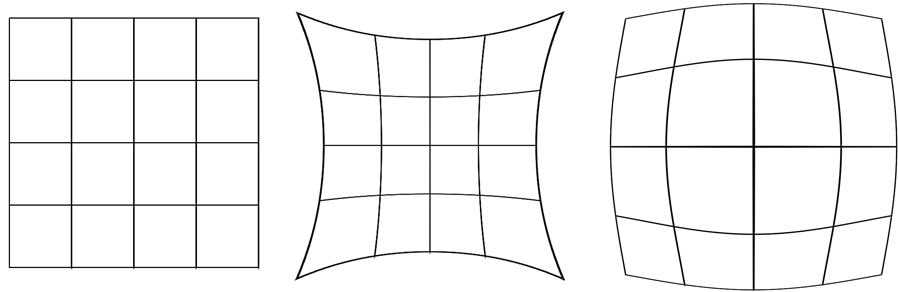
\includegraphics[width=1\linewidth]{images/lens} \caption{Les differentes types de distortion. Du gauche à la droit : la grille d'origine, la distorsion en barillet et la distorsion en coussinet.}\label{fig:lens}
\end{figure}

Les formules suivantes sont appliquées pour supprimer la distortion radial (Voir Équation\eqref{eq:corr1}) et la distorsion tangentielle (Voir Équation\eqref{eq:corr2})

\begin{equation}
\begin{aligned}
  x_{corr} = x\left(1+k_1r^2+k_2r^4+k_3r^6\right)
  \\y_{corr} = y\left(1+k_1r^2+k_2r^4+k_3r^6\right)
\end{aligned}
 \label{eq:corr1}
\end{equation}

D'où \(𝑥\) et \(𝑦\) sont les coordonnées d'origine; \(x_{𝑐𝑜𝑟𝑟}\) et
\(y_{𝑐𝑜𝑟𝑟}\) sont les coordonnées corrigés. \(𝑟\) est la distance entre le
point \(\left(𝑥, 𝑦\right)\) et le centre de la distortion. \(𝑘_1\), \(𝑘_2\),
et \(𝑘_3\) sont les coefficients radiales. Pour la distortion en barillet et la distortion en coussinet , \(𝑘_1\) est respectivemen negative et positive. \(𝑘_2\) et \(𝑘_3\) sont négligeables.

\begin{equation}
\begin{aligned}
   x_{corr} = x+\left[ 2 p_1 x y+ p_2\left( r^2+2x^2\right) \right]\\
  y_{corr} = y+\left[ p_1 \left(r^2+2 y^2\right)+ 2p_2xy\right]
\end{aligned}
 \label{eq:corr2}
\end{equation}

D'où \(𝑝_1\) et \(𝑝_2\) sont les coefficient de la distortion tangentielle. les différents coefficients sont souvent stockés dans un tableau:

\begin{equation}
C_{dis}=
\begin{bmatrix}
k_1 & k_2 & p_1 & p_2 & k_3
\end{bmatrix}
\end{equation}

À part du coefficient de distorsion, pour pouvoir corriger l'imagerie, Une conversion entre les coordonnées de distorsion et la résolution de la caméra est
fait. Pour cela, la formule est donnée dans l'équation \eqref{eq:corr3}

\begin{equation}
\begin{bmatrix}
x\\
y\\
w
\end{bmatrix}
= M_{con} \cdot
\begin{bmatrix}
x\\
y\\
z
\end{bmatrix}
\quad d'où \quad
M_{con} =
\begin{bmatrix}
f_x & 0 & c_x\\
0 & f_y & x_y\\
0 & 0 &1
\end{bmatrix}
\label{eq:corr3}
\end{equation}

D'où \([𝑥, 𝑦, 𝑤]\) sont les coordonnées d'image homogène 2D et \([x, y , z]\) sont les coordonnées de caméra 3D . \(f_𝑥\) et \(𝑓_𝑦\) sont les longueurs locales de la caméra dans le sens \(𝑥\) et \(𝑦\) ,en genéral, ils sont identiques - \(𝑐_𝑥\) et \(𝑐_𝑦\) sont les coordinations de centre optique de la caméra dans le sens \(𝑥\) et \(𝑦\).

\hypertarget{la-stabilisation}{%
\subsubsection*{La stabilisation}\label{la-stabilisation}}
\addcontentsline{toc}{subsubsection}{La stabilisation}

Après avoir appliqué la correction de la distorsion optique , le mouvements d'images possibles
peut être supprimé en appliquant la stabilisation de vidéo. Les principales étapes de
stabilisation sont (1) l'extraction de points clés sur deux trames séquentielles,
(2) faire correspondre les points sur les deux trames, (3) estimer le
transformation géométrique, et (4) correction du mouvement.

\hypertarget{lorthorectification-dimage}{%
\subsubsection*{l'orthorectification d'image}\label{lorthorectification-dimage}}
\addcontentsline{toc}{subsubsection}{l'orthorectification d'image}

Pour supprimer les effets de la perspective de l'image -- là où les objets sont plus proches
de la caméra semble être plus grande que les objets en arrière-plan -- ,
l'orthorectification est appliquée. Lors de l'application d'orthorectification,
le système de coordonnées de l'imagerie est transféré à une coordonnée locale
système. Pour ce système de coordonnées locales, points de contrôle au sol (GCP) --
mis en place à côté du flux -- sont utilisés. Pour l'orthorectification
processus pour être aussi précis que possible, au moins quatre GCP sont nécessaires, si
les images sont capturées perpendiculairement au flux ou lorsque les GCP
sont placés au même niveau que le niveau de l'eau. Un minimum de six
GCP sont nécessaires lorsque les GCP ne sont pas placés dans le même plan que le
niveau d'eau. Sur la Figure \ref{fig:ortho} les différents sites de jaugeage
et les configurations sont affichées.



\begin{figure}
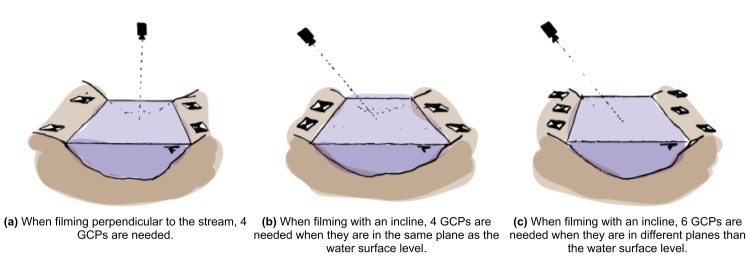
\includegraphics[width=1\linewidth]{images/ortho} \caption{Nombre de points de contrôle au sol (GCP) nécessaires dans différentes circonstances.}\label{fig:ortho}
\end{figure}

Lors de l'utilisation de quatre GCP, les facteurs d'inversion \(𝑓_𝑥\) et \(𝑓_𝑦\) sont
déterminé en utilisant la formule indiquée dans l'équation \eqref{eq:corr4}.

\begin{equation}
p_{loc}\left(x,y\right)=p_{img}\left(f_x\left(x,y\right), f_y\left(x,y\right)\right)
\label{eq:corr4}
\end{equation}

D'où \(𝑝_ {𝑑𝑠𝑡} \left (𝑥, 𝑦, 𝑧 \right)\) est l'emplacement géographique du
point de contrôle au sol dans le système de coordonnées local, généralement en métrique
units; \(𝑝_ {𝑠𝑟𝑐} \left (𝑥, 𝑦 \right)\) est la coordonnée xy du sol
point de contrôle dans l'imagerie, généralement en pixels; et \(𝑓_𝑥\) et \(𝑓_𝑦\) le
facteurs d'inversion.

Simultanément à ce processus, la résolution de l'image peut être réglée
en multipliant les coordonnées \(𝐺𝐶𝑃_ {𝑑𝑠𝑡} \left (𝑥, 𝑦 \right)\) par les
pixels souhaités par coefficient de mètre. Un exemple de
le processus d'orthorectification est illustré à la Figure \ref{fig:orthoafter} .



\begin{figure}
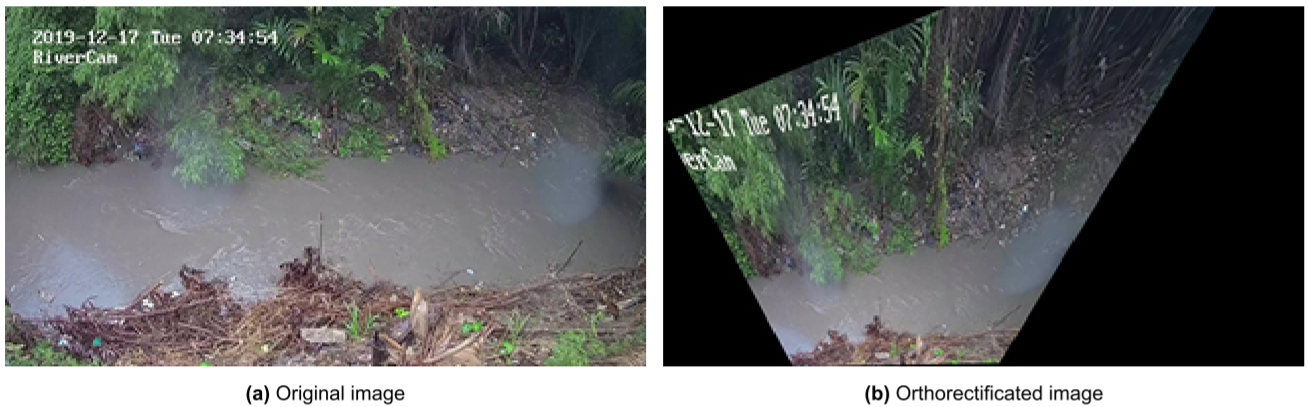
\includegraphics[width=1\linewidth]{images/ortho_after} \caption{Exemple de processus d'orthorectification utilisant quatre GCP, indiqués par des poteaux en bambou le long du ruisseau.}\label{fig:orthoafter}
\end{figure}

Lorsque six (ou plus) GCP sont utilisés - parce que les coordonnées en trois dimensions
pour les GCP sont nécessaires - un modèle de sténopé peut être utilisé. Cette méthode est
expliqué par \citep{jodeau_application_2008} .

\hypertarget{la-mise-en-niveau-de-gris-et-la-correction-du-gamma-et-du-contraste}{%
\subsubsection*{La mise en niveau de gris et la correction du gamma et du contraste}\label{la-mise-en-niveau-de-gris-et-la-correction-du-gamma-et-du-contraste}}
\addcontentsline{toc}{subsubsection}{La mise en niveau de gris et la correction du gamma et du contraste}

La dernière étape de la préparation de l'image est la conversion du
imagerie à une échelle de gris et pour appliquer une correction de contraste et gamma.
Une mise à l'échelle des gris est nécessaire pour pouvoir appliquer la validation de similarité entre
images vidéo séquentielles. La correction de contraste et gamma est appliquée à
améliorer la visibilité des semences. Les corrections de contraste et gamma sont
appliqué à l'aide des formules suivantes:

\begin{equation}
O_{constract} = \alpha \cdot I + \beta
\label{eq:constract}
\end{equation}

\begin{equation}
O_{gamma} = \left(\frac{I}{255}\right)^\frac{1}{\gamma} \cdot 255
\label{eq:gamma}
\end{equation}

where \(\alpha\) and \(\beta\) defines the contrast correction; \(\gamma\) the
gamma correction; \(O_n\) are the corrected imagery; and \(I\) is the
original imagery

D'où \(\alpha\) et \(\beta\) définit la correction du contraste; \(\gamma\) est la correction de gamma; \(O_n\) sont les imageries corrigés; et \(I\) est l'imagerie d'origine.

\hypertarget{pp}{%
\subsection{PIV processing}\label{pp}}

La figure \ref{fig:pivprocessing} montre les étapes du traitement PIV. Pour deux séquentiels
cadres, les images sont divisées en cellules de grille. En déterminant
validation de similarité - par exemple, une corrélation croisée ou une
rapport signal / bruit \citetext{\citealp[ ]{ran_application_2016}; \citealp{osorio-cano_method_2013}} -
entre les deux cadres de la zone de recherche, les déplacements peuvent être
déterminé. Ces déplacements sont ensuite convertis en vitesse d'écoulement
vecteurs.

Après avoir appliqué ce processus sur \(𝑁\) images, un total de \(𝑁− 1\) cartes de vitesse
sont créées. Pour chaque carte de vitesse, les résultats peuvent être encore améliorés
en appliquant un filtrage supplémentaire basé sur la valeur de similarité dans chaque
fenêtre d'interrogation unique, et en remplaçant ces valeurs filtrées par
interpolation les cellules de la grille environnantes connues. Ces post-traitements
les étapes dépendent du logiciel utilisé ou des résultats requis.



\begin{figure}
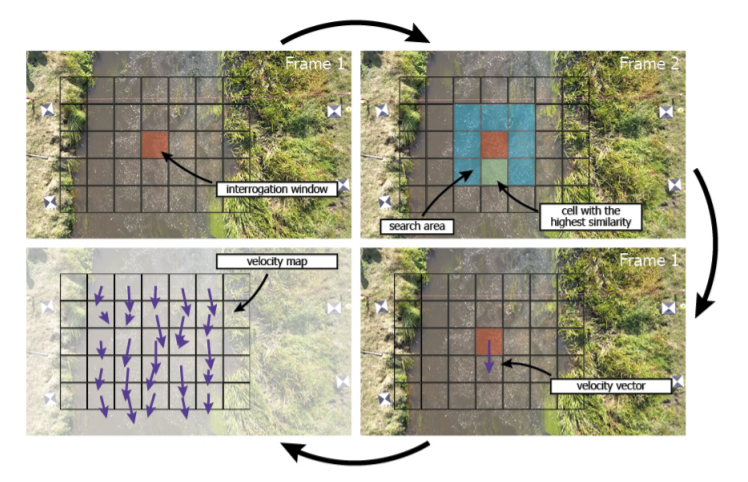
\includegraphics[width=1\linewidth]{images/pivprocessing} \caption{Vue schématique de la méthode LSPIV où une fenêtre d'interrogation est déterminée (la grille est dessinée plus grande dan généralement appliqué) dans la première image et les graines présentes sont comparées à une zone de recherche dans l'image séquentielle 2 à déterminer leurs déplacements. En multipliant le déplacement par la période de temps de trame, la vitesse est déterminée. Lorsque vous appliquez ceci sur toute l'image, une carte de vitesse d'écoulement de surface peut être créée pour chaque image individuelle.}\label{fig:pivprocessing}
\end{figure}

\newpage

  \bibliography{LSPIV.bib}

\end{document}
